% -*- Mode: LaTeX; Package: CLIM-USER -*-

\chapter {Bounding Rectangles}
\label {bboxes}

\section {Bounding Rectangles}

Every bounded region has a derived \concept{bounding rectangle}, which is a
rectangular region whose sides are parallel to the coordinate axes.  Therefore,
every bounded region participates in the bounding rectangle protocol.  The
bounding rectangle for a region is the smallest rectangle that contains every
point in the region.  However, the bounding rectangle may contain additional
points as well.  Unbounded regions do not have a bounding rectangle and do not
participate in the bounding rectangle protocol.  Other objects besides bounded
regions participate in the bounding rectangle protocol, such as sheets and
output records.

The coordinate system in which the bounding rectangle is maintained depends on
the context.  For example, the coordinates of the bounding rectangle of a sheet
are expressed in the sheet's parent's coordinate system.  For output records,
the coordinates of the bounding rectangle are maintained in the coordinate
system of the stream with which the output record is associated.

Note that the bounding rectangle of a transformed region is not in general the
same as the result of transforming the bounding rectangle of a region, as shown
in Figure~\ref{output-record-bbox}.  For transformations that satisfy
\cl{rectilinear-transformation-p}, the following equality holds.  For all other
transformations, it does not hold.

\begin{verbatim}
(region-equal
  (transform-region transformation (bounding-rectangle region))
  (bounding-rectangle (transform-region transformation region)))
\end{verbatim}

\begin{figure}
\centerline{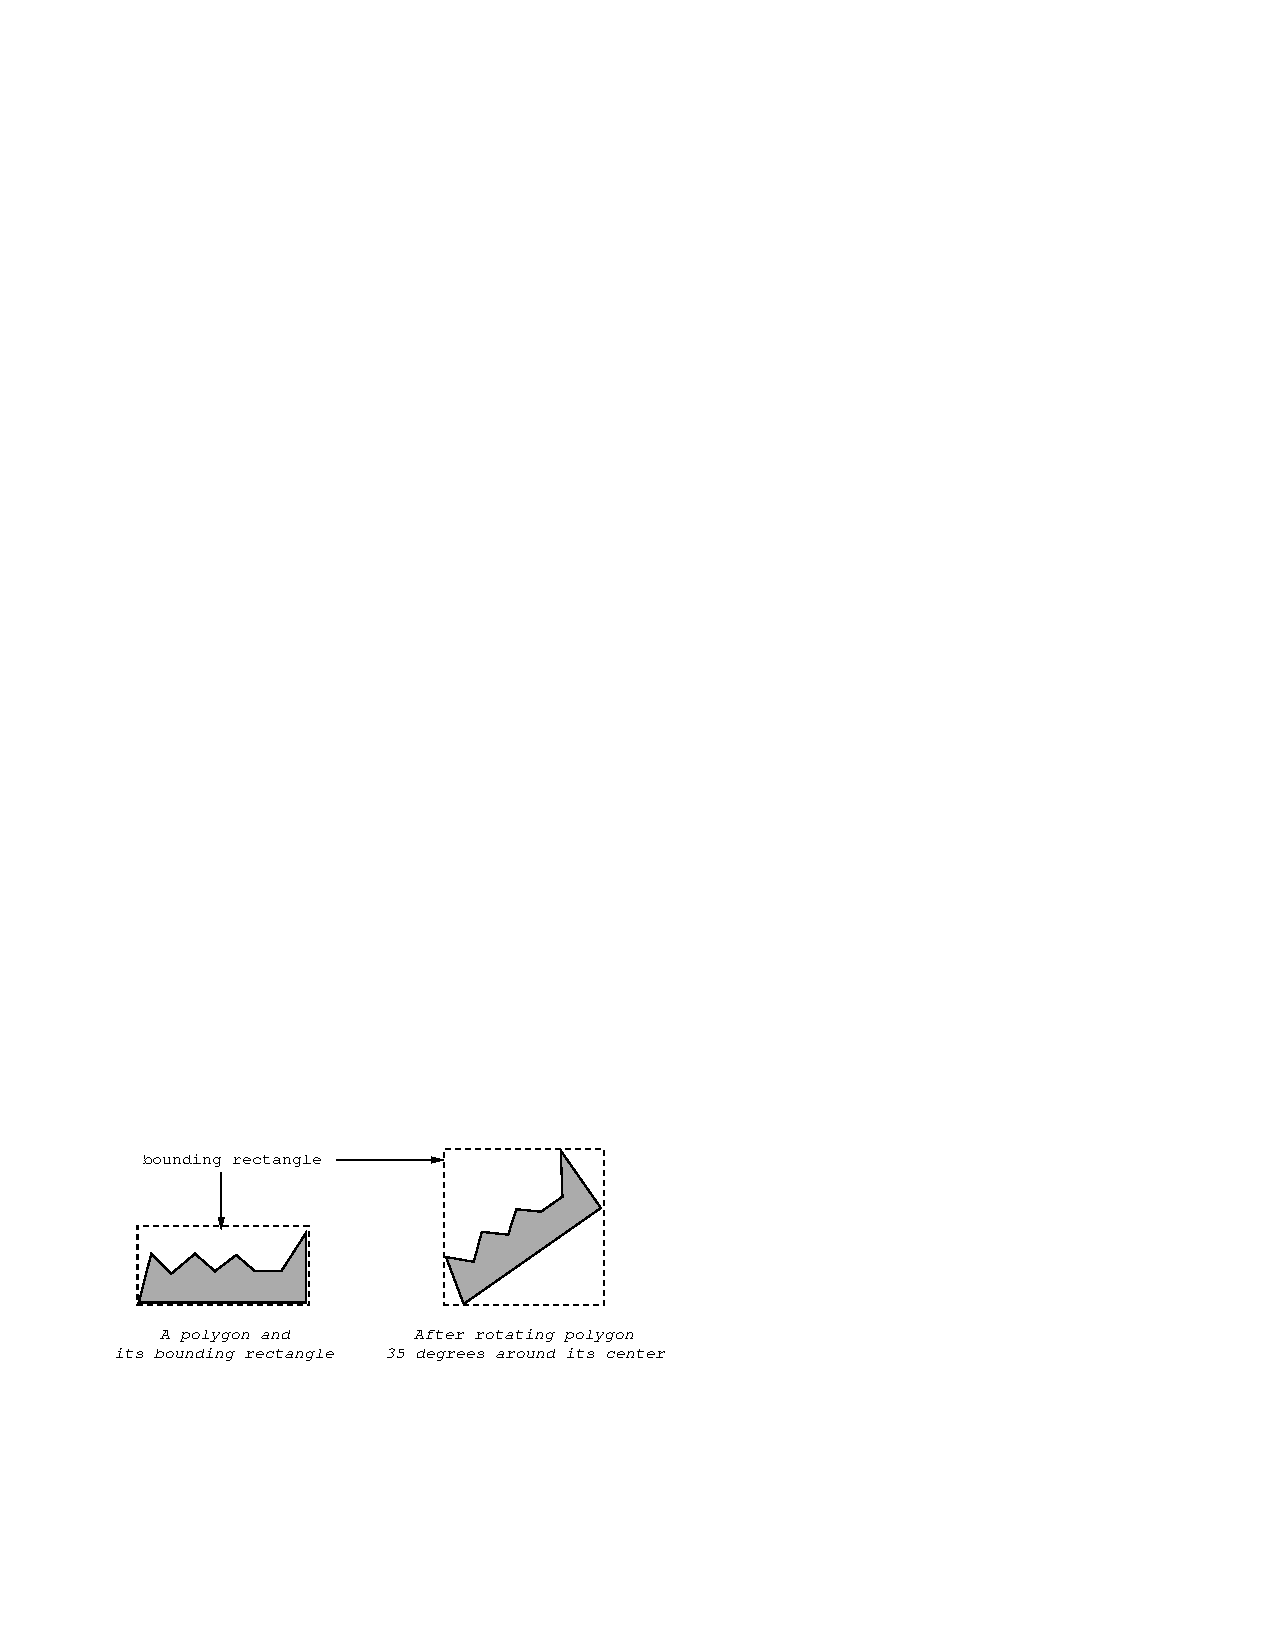
\includegraphics{bounding-box}}
\caption{\label{output-record-bbox} The bounding rectangle of an output record.}
\end{figure}

CLIM uses bounding rectangles for a variety of purposes.  For example,
repainting of windows is driven from the bounding rectangle of the window's
viewport, intersected with a ``damage'' region.  The formatting engines used by
\cl{formatting-table} and \cl{formatting-graph} operate on the bounding
rectangles of the output records in the output.  Bounding rectangles are also
used internally by CLIM to achieve greater efficiency.  For instance, when
performing hit detection to see if the pointer is within the region of an output
record, CLIM first checks to see if the pointer is within the bounding rectangle
of the output record.

Note that the bounding rectangle for an output record may have a different size
depending on the medium on which the output record is rendered.  Consider the
case of rendering text on different output devices; the font chosen for a
particular text style may vary considerably in size from one device to another.

\Defprotoclass {bounding-rectangle}

The protocol class that represents a bounding rectangle.
\IfYouWantClass {a} {bounding rectangle} {bounding-rectangle}

Note that bounding rectangles are not a subclass of \cl{rectangle}, nor even a
subclass of \cl{region}.  This is because, in general, bounding rectangles do
not obey the region protocols.  However, all bounded regions and sheets that
obey the bounding rectangle protocol are subclasses of \cl{bounding-rectangle}.

Bounding rectangles are immutable, but since they reflect the live state of such
mutable objects as sheets and output records, bounding rectangles are volatile.
Therefore, programmers must not depend on the bounding rectangle associated with
a mutable object remaining constant.

\Defpredicate {bounding-rectangle-p} {object}

Returns \term{true} if \arg{object} is a \term{bounding rectangle} (that is,
supports the bounding rectangle protocol), otherwise returns \term{false}.

\Defclass {standard-bounding-rectangle}

An instantiable class that implements a bounding rectangle.  This is a subclass
of both \cl{bounding-rectangle} and \cl{rectangle}, that is, standard bounding
rectangles obey the rectangle protocol.

\cl{make-bounding-rectangle} returns an object of this class.

The representation of bounding rectangles in CLIM is chosen to be efficient.
CLIM will probably represent such rectangles by storing the coordinates of two
opposing corners of the rectangle, namely, the ``min point'' and the ``max
point''.  Because this representation is not sufficient to represent the result
of arbitrary transformations of arbitrary rectangles, CLIM is allowed to return
a polygon as the result of such a transformation.  (The most general class of
transformations that is guaranteed to always turn a rectangle into another
rectangle is the class of transformations that satisfy
\cl{rectilinear-transformation-p}.)

\Defun {make-bounding-rectangle} {x1 y1 x2 y2}

Returns an object of the class \cl{standard-bounding-rectangle} with the edges
specified by \arg{x1}, \arg{y1}, \arg{x2}, and \arg{y2}, which must be real
numbers.

\arg{x1}, \arg{y1}, \arg{x2}, and \arg{y2} are ``canonicalized'' in the
following way.  The min point of the rectangle has an $x$ coordinate that is the
smaller of \arg{x1} and \arg{x2} and a $y$ coordinate that is the smaller of
\arg{y1} and \arg{y2}.  The max point of the rectangle has an $x$ coordinate
that is the larger of \arg{x1} and \arg{x2} and a $y$ coordinate that is the
larger of \arg{y1} and \arg{y2}.  (Therefore, in a right-handed coordinate
system the canonicalized values of \arg{x1}, \arg{y1}, \arg{x2}, and \arg{y2}
correspond to the left, top, right, and bottom edges of the rectangle,
respectively.)

\FreshOutputs


\subsection {The Bounding Rectangle Protocol}

The following generic function comprises the bounding rectangle protocol.  All
classes that participate in this protocol (including all subclasses of
\cl{region} that are bounded regions) must implement a method for
\cl{bounding-rectangle*}.

\Defgeneric {bounding-rectangle*} {region}

Returns the bounding rectangle of \arg{region} as four real numbers specifying
the $x$ and $y$ coordinates of the min point and the $x$ and $y$ coordinates of
the max point of the rectangle.  The argument \arg{region} must be either a
bounded region (such as a line or an ellipse) or some other object that obeys
the bounding rectangle protocol, such as a sheet or an output record.

The four returned values \arg{min-x}, \arg{min-y}, \arg{max-x}, and \arg{max-y}
will satisfy the inequalities
\begin{eqnarray*}
  minx \leq maxx \\
  miny \leq maxy \\
\end{eqnarray*}


\Defgeneric {bounding-rectangle} {region}

Returns the bounding rectangle of \arg{region} as an object that is a subclass
of \cl{rectangle} (described in Section~\ref{rect}).  The argument \arg{region}
must be either a bounded region (such as a line or an ellipse) or some other
object that obeys the bounding rectangle protocol, such as a sheet or an output
record.

It is unspecified whether \cl{bounding-rectangle} will or will not create a new
object each time it is called.  Many CLIM implementations will cache the
bounding rectangle for sheets and output records.  The implication of this is
that, since bounding rectangles are volatile, programmers should depend on the
object returned by \cl{bounding-rectangle} remaining constant.

\cl{bounding-rectangle} is part of the bounding rectangle API, but not part of
the bounding rectangle protocol.  CLIM will supply a default method for
\cl{bounding-rectangle} on the protocol class \cl{bounding-rectangle} that is
implemented by calling \cl{bounding-rectangle*}.


\subsection {Bounding Rectangle Convenience Functions}

The functions described below are part of the bounding rectangle API, but are
not part of the bounding rectangle protocol.  They are provided as a convenience
to programmers who wish to specialize classes that participate in the bounding
rectangle protocol, but do not complicate the task of those programmers who
define their own types (such as sheet classes) that participate in this
protocol.

CLIM will supply default methods for all of these generic functions on the
protocol class \cl{bounding-rectangle} that are implemented by calling
\cl{bounding-rectangle*}.


\Defmacro {with-bounding-rectangle*} {(min-x min-y max-x max-y) region \body body}  

Binds \arg{min-x}, \arg{min-y}, \arg{max-x}, and \arg{max-y} to the edges of the
bounding rectangle of \arg{region}, and then executes \arg{body} in that
context.  The argument \arg{region} must be either a bounded region (such as a
line or an ellipse) or some other object that obeys the bounding rectangle
protocol, such as a sheet or an output record.

The arguments \arg{min-x}, \arg{min-y}, \arg{max-x}, and \arg{max-y} are not
evaluated.  \arg{body} may have zero or more declarations as its first forms.

\cl{with-bounding-rectangle*} must be implemented by calling \cl{bounding-rectangle*}.


\Defgeneric {bounding-rectangle-position} {region}

Returns the position of the bounding rectangle of \arg{region}.  The position of
a bounding rectangle is specified by its min point.


\defgeneric {bounding-rectangle-min-x} {region}
\defgeneric {bounding-rectangle-min-y} {region}
\defgeneric {bounding-rectangle-max-x} {region}
\Defgeneric {bounding-rectangle-max-y} {region}

Returns (respectively) the $x$ and $y$ coordinates of the min point and the $x$
and $y$ coordinate of the max point of the bounding rectangle of \arg{region}.
The argument \arg{region} must be either a bounded region or some other object
that obeys the bounding rectangle protocol.


\defgeneric {bounding-rectangle-width}  {region}
\defgeneric {bounding-rectangle-height} {region}
\Defgeneric {bounding-rectangle-size}   {region}

Returns the width, height, or size (as two values, the width and height) of the
bounding rectangle of \arg{region}, respectively.  The argument \arg{region}
must be either a bounded region or some other object that obeys the bounding
rectangle protocol.

The width of a bounding rectangle is the difference between its maximum $x$
coordinate and its minimum $x$ coordinate.  The height is the difference between
the maximum $y$ coordinate and its minimum $y$ coordinate.
